
This section discusses the user selection schemes discussed in sections \ref{sus} and \ref{cus}. The users are assumed to be located at the cell-edge and the objective is to maximize the achievable capacity of the system. The precoding schemes considered here are based on combined zero-forcing with water-filling (CZF-WF) and W-MMSE based joint precoding and scheduling design discussed in \cite{wmmse_shi}. The W-MMSE scheme performs joint precoding and scheduling of users with the maximizing sum capacity objective. The ZF scheme performs only precoder design for the users in \me{\mc{S}_b} which mandates the users to be selected in way to maximize the sum capacity. The selection of users for multi-BS system needs to be exhaustive in order to achieve the capacity attaining user set \me{\mc{S}_b}. The static user scheduling (SUS) and coordinated user scheduling (CUS) provides one such approach in which users can be selected with minimal complexity in comparison with the exhaustive user search. The user selection schemes discussed earlier provides the better transmission set compared with the conventional user selection scheme for sum rate objective.
\begin{figure}[hb]
\centering
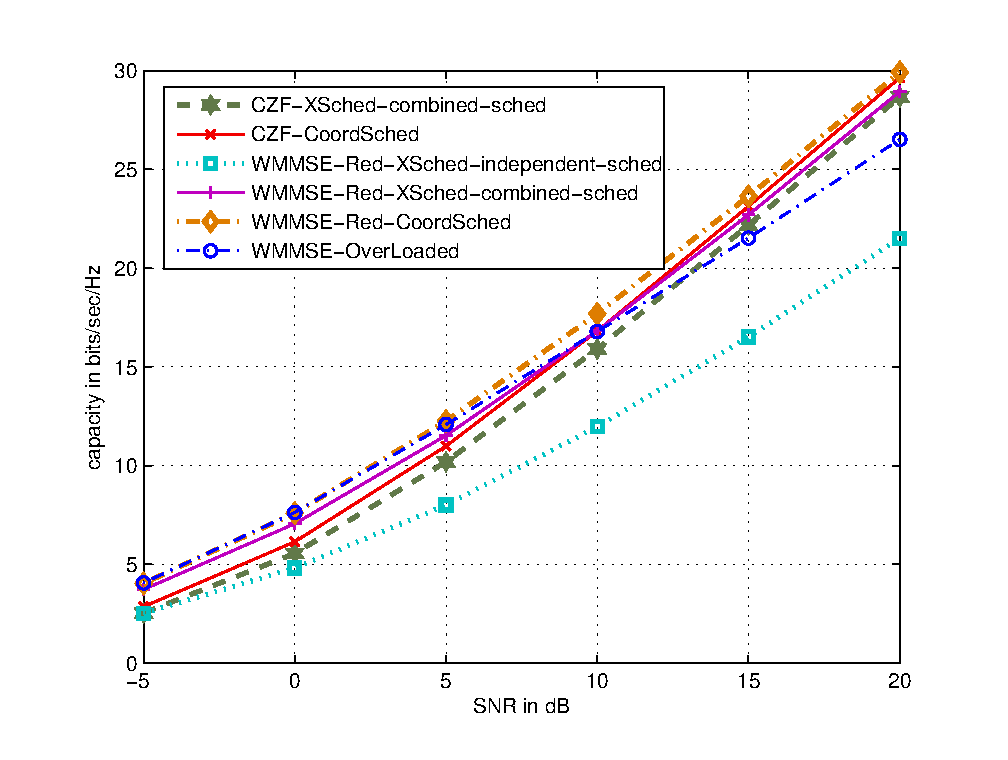
\includegraphics[width=0.8\textwidth]{multi-bs-1}
\caption[short]{Sum capacity for \me{\card{\mc{B}} = 2, \, \card{\mc{U}_k} = 25, \, N_\mrm{T} = 4, \, N_\mrm{R} = 1}}
\label{multi-bs-f1}
\end{figure}

Fig. \ref{multi-bs-f1} shows the comparison of the above mentioned schemes using CZF-WF and W-MMSE precoding designs. The CZF-WF based design is equivalent to W-MMSE scheme at higher SNR when the transmission user set \me{\mc{S}_b} is defined. The reduced W-MMSE scheme is performed over the transmission user set \me{\mc{S}_b \fall b \inm \mc{B}} in contrast with the overloaded W-MMSE scheme performing over the entire user set \me{\mc{U}_b}. The performance of the overloaded W-MMSE scheme degrades as the SNR increases to that of reduced W-MMSE scheme with SUS based user selection for the same stopping resolution \me{\epsilon} as defined in \cite{wmmse_shi}. Even though overloaded W-MMSE performs better at lower SNRs, the reduced W-MMSE using SUS based user selection provides significantly improved performance at higher SNR owing to the fact of reduced variables involved in the optimization problem. The variable reduction is mainly achieved by the selection scheme performed using SUS.

Fig. \ref{multi-bs-f1} plots the performance of CUS scheme as well in comparison with SUS schemes using W-MMSE over reduced user set obtained by the selection algorithms. The CUS scheme provides improved performance by selecting users over the entire user set \me{\mc{U}} for all BSs in \me{\mc{B}} instead selecting over \me{\mc{U}_b} for BS \me{b \fall b \inm{\mc{B}}}. The CUS scheme avails the additional multi-user selection diversity over conventional SUS based schemes to achieve significant performance improvement. The CUS performance is limited by the number of users available for selection since more users in \me{\mc{U}_b}, more diverse users in the set thereby SUS also enjoys more multi-user diversity performing closer to CUS scheme. To achieve any gain from CUS scheme over SUS scheme, the user set \me{\mc{U}} over which the scheduling is performed should be at the cell-edge thereby availing the instantaneous fading for scheduling users.
\begin{figure}
\centering
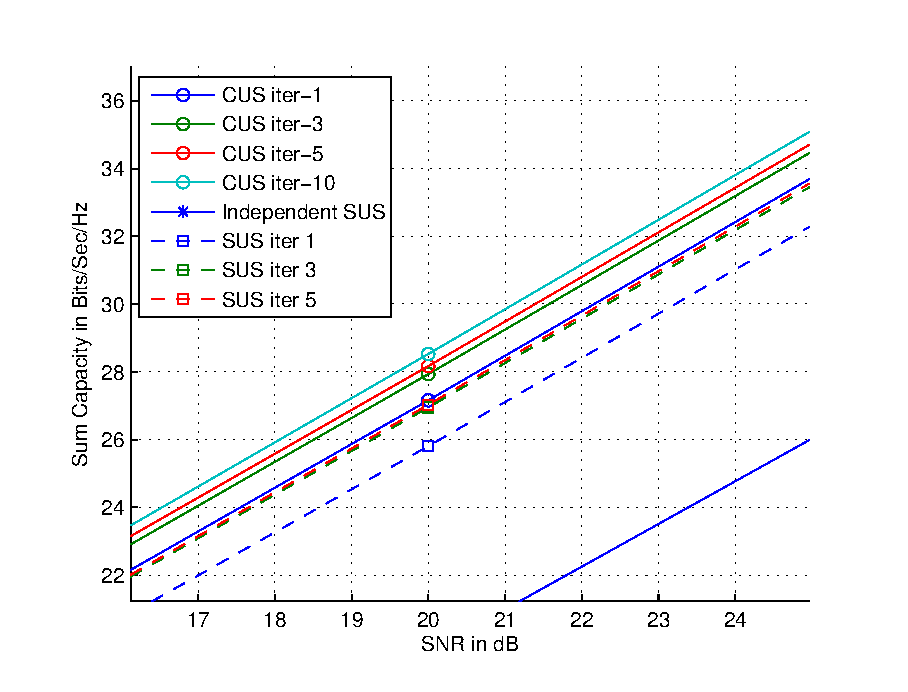
\includegraphics[trim = 0cm 0cm 0cm 7mm, clip, width=0.8\textwidth]{multi-bs-2}
\caption[short]{Iterative sum capacity for \me{\card{\mc{B}} = 2, \, \card{\mc{U}} = 20, \, N_\mrm{T} = 4, \, N_\mrm{R} = 1}}
\label{multi-bs-f2}
\end{figure}

Fig. \ref{multi-bs-f2} depicts the iterative performance improvement of CUS and SUS schemes for different iteration count using sum capacity as the metric. Since the search space is bounded by the user sets \me{\mc{U}, \: \mc{U}_b}, the performance at each iteration will be monotonic in terms of sum rate objective. The selected set at each iterations will be at least good as the earlier transmission user set \me{\mc{S}_b} but not inferior in terms of sum rate metric as shown in Fig. \ref{multi-bs-f2}.
